% Options for packages loaded elsewhere
\PassOptionsToPackage{unicode}{hyperref}
\PassOptionsToPackage{hyphens}{url}
%
\documentclass[
  ignorenonframetext,
]{beamer}
\usepackage{pgfpages}
\setbeamertemplate{caption}[numbered]
\setbeamertemplate{caption label separator}{: }
\setbeamercolor{caption name}{fg=normal text.fg}
\beamertemplatenavigationsymbolsempty
% Prevent slide breaks in the middle of a paragraph
\widowpenalties 1 10000
\raggedbottom
\setbeamertemplate{part page}{
  \centering
  \begin{beamercolorbox}[sep=16pt,center]{part title}
    \usebeamerfont{part title}\insertpart\par
  \end{beamercolorbox}
}
\setbeamertemplate{section page}{
  \centering
  \begin{beamercolorbox}[sep=12pt,center]{part title}
    \usebeamerfont{section title}\insertsection\par
  \end{beamercolorbox}
}
\setbeamertemplate{subsection page}{
  \centering
  \begin{beamercolorbox}[sep=8pt,center]{part title}
    \usebeamerfont{subsection title}\insertsubsection\par
  \end{beamercolorbox}
}
\AtBeginPart{
  \frame{\partpage}
}
\AtBeginSection{
  \ifbibliography
  \else
    \frame{\sectionpage}
  \fi
}
\AtBeginSubsection{
  \frame{\subsectionpage}
}
\usepackage{lmodern}
\usepackage{amssymb,amsmath}
\usepackage{ifxetex,ifluatex}
\ifnum 0\ifxetex 1\fi\ifluatex 1\fi=0 % if pdftex
  \usepackage[T1]{fontenc}
  \usepackage[utf8]{inputenc}
  \usepackage{textcomp} % provide euro and other symbols
\else % if luatex or xetex
  \usepackage{unicode-math}
  \defaultfontfeatures{Scale=MatchLowercase}
  \defaultfontfeatures[\rmfamily]{Ligatures=TeX,Scale=1}
\fi
% Use upquote if available, for straight quotes in verbatim environments
\IfFileExists{upquote.sty}{\usepackage{upquote}}{}
\IfFileExists{microtype.sty}{% use microtype if available
  \usepackage[]{microtype}
  \UseMicrotypeSet[protrusion]{basicmath} % disable protrusion for tt fonts
}{}
\makeatletter
\@ifundefined{KOMAClassName}{% if non-KOMA class
  \IfFileExists{parskip.sty}{%
    \usepackage{parskip}
  }{% else
    \setlength{\parindent}{0pt}
    \setlength{\parskip}{6pt plus 2pt minus 1pt}}
}{% if KOMA class
  \KOMAoptions{parskip=half}}
\makeatother
\usepackage{xcolor}
\IfFileExists{xurl.sty}{\usepackage{xurl}}{} % add URL line breaks if available
\IfFileExists{bookmark.sty}{\usepackage{bookmark}}{\usepackage{hyperref}}
\hypersetup{
  pdftitle={Tema 4 - Variables Aleatorias continuas multidimensionales},
  pdfauthor={Ricardo Alberich, Juan Gabriel Gomila y Arnau Mir},
  hidelinks,
  pdfcreator={LaTeX via pandoc}}
\urlstyle{same} % disable monospaced font for URLs
\newif\ifbibliography
\setlength{\emergencystretch}{3em} % prevent overfull lines
\providecommand{\tightlist}{%
  \setlength{\itemsep}{0pt}\setlength{\parskip}{0pt}}
\setcounter{secnumdepth}{-\maxdimen} % remove section numbering

\title{Tema 4 - Variables Aleatorias continuas multidimensionales}
\author{Ricardo Alberich, Juan Gabriel Gomila y Arnau Mir}
\date{}

\begin{document}
\frame{\titlepage}

\hypertarget{variables-aleatorias-bidimensionales-continuas}{%
\section{Variables aleatorias bidimensionales
continuas}\label{variables-aleatorias-bidimensionales-continuas}}

\begin{frame}{Variables aleatorias bidimensionales continuas
Introducción}
\protect\hypertarget{variables-aleatorias-bidimensionales-continuas-introducciuxf3n}{}
Definición de variable aleatoria bidimensional continua.

Recordemos que una v.a. bidimensional \textbf{continua} cuando su
conjunto de valores en \(\mathbb{R}^2\), \((X,Y)(\Omega)\) es un
producto de intervalos.

Definición función de distribución conjunta

La función de distribución acumulada conjunto o simplemente distribución
conjunta se define como

\[F_{XY}(x,y)=P(X\leq x,Y\leq y).\]
\end{frame}

\begin{frame}{Función de distribución acumulada función de densidad}
\protect\hypertarget{funciuxf3n-de-distribuciuxf3n-acumulada-funciuxf3n-de-densidad}{}
Definición función de densidad conjunta

Sea \(f_{XY}: \mathbb{R}\times \mathbb{R}\mapsto [0,+\infty)\) diremos
que es una densidad bidimensional del vector aleatorio bidimensional
\((X,Y)\) si

\[F_{XY}(x,y)=\int_{-\infty}^{x}\int_{-\infty}^{y} f_{XY}(t_x,t_y) dt_xdt_y.\]

Llamaremos dominio de la variable conjunta a
\[D_{XY}=\{(x,y)\in \mathbb{R}^2 | f_{XY}(x,y)>0\}.\]

Es decir es el conjunto de valores posibles que toma la v.a. \((X,Y)\).
\end{frame}

\begin{frame}{Propiedades de la función de densidad conjunta}
\protect\hypertarget{propiedades-de-la-funciuxf3n-de-densidad-conjunta}{}
Sea \((X,Y)\) una \textbf{variable aleatoria bidimensional continua} con
dominio \(D_{XY}\subset \mathbb{R}^2\).

Su \textbf{función de densidad conjunta} verifica las siguientes
propiedades:

\begin{itemize}
\item
  \[\int_{-\infty}^{+\infty} f_{XY}(x,y)\quad  dx dy=1.\]
\item
  Sea \(B\) un subconjunto cualquiera del dominio \(D_{XY}\). El valor
  de la probabilidad \(P((X,Y)\in B)\) se puede calcular de la forma
  siguiente: \[
  P((X,Y)\in B) ={\int\int}_B f_{XY}(x,y)\quad  dx dy=1.
  \]
\end{itemize}

Es decir, la probabilidad de que la variable bidimensional tome valores
en \(B\) es igual al volumen que genera la densidad conjunta sobre el
recinto \(B\).
\end{frame}

\hypertarget{distribuciones-marginales}{%
\section{Distribuciones marginales}\label{distribuciones-marginales}}

\begin{frame}{Variables aleatorias marginales y su distribución}
\protect\hypertarget{variables-aleatorias-marginales-y-su-distribuciuxf3n}{}
Consideremos una variable aleatoria \textbf{bidimensional continua
\((X,Y)\)} con \textbf{función de probabilidad conjunta} \(f_{XY}(x,y)\)
y coon domicio \(D_{XY}\).

La tabla de la \textbf{función de densidad conjunta} contiene suficiente
información para obtener las \textbf{funciones de densidad} de las
variables \(X\) e \(Y\).

Dichas variables \(X\) e \(Y\) se denominan \textbf{variables
marginales} y sus correspondientes \textbf{funciones de densidad},
\textbf{funciones de densidad marginales} \(f_X\) de la variable \(X\) y
\(f_Y\) de la variable \(Y\).

Veamos cómo obtener \(f_X\) y \(f_Y\) a partir de la tabla \(f_{XY}\).
\end{frame}

\begin{frame}{Funciones de probabilidad marginales}
\protect\hypertarget{funciones-de-probabilidad-marginales}{}
Proposición. Cálculo de las funciones de densidad marginales.

Sea \((X,Y)\) una variable aleatoria \textbf{bidimensional continua} con
\textbf{función de densidad conjunta} \(f_{XY}(x,y)\), con
\((x,y)\in D_{XY}\).

Las \textbf{funciones de densidad marginales} \(f_X(x)\) y \(f_Y(y)\) se
calculan usando las expresiones siguientes:

\begin{itemize}
\item
  \(f_X(x)= \displaystyle \int_{-\infty}^{+\infty} f(x,y)\quad dy.\)
\item
  \(f_Y(y)= \displaystyle \int_{-\infty}^{+\infty} f(x,y)\quad dx.\)
\end{itemize}
\end{frame}

\begin{frame}{Independencia de variables aleatorias continuas}
\protect\hypertarget{independencia-de-variables-aleatorias-continuas}{}
Recordemos que dos sucesos \(A\) y \(B\) son independientes si

\[P(A\cap B)=P(A)\cdot P(B).\]

¿Cómo trasladar dicho concepto al caso de variables aleatorias
continuas?

Dada una variable aleatoria bidimensional continua \((X,Y)\) con dominio
\(D_{XY}\)

Así que al menos todos los sucesos de la forma
\(P\left(X\leq x_i,\  Y\leq y\right)\) deberán ser independientes. Esto
implicará que cualesquiera dos sucesos de cada variables con
inpedendientes.
\end{frame}

\begin{frame}{Independencia de variables aleatorias continuas}
\protect\hypertarget{independencia-de-variables-aleatorias-continuas-1}{}
Condiciones para independencia de variables aleatorias bidimensionales
continuas

Dada \((X,Y)\) una \textbf{variable aleatoria bidimensional continua}
con \textbf{función de densidad} \(f_{XY}\) y \textbf{funciones de
probabilidad marginales} \(f_X\) y \(f_Y\).

Diremos que \(X\) e \(Y\) son independientes si se cumple al menos una
de las siguientes condiciones:

\begin{itemize}
\item
  \(f_{XY}(x,y)=f_X(x)\cdot f_Y(y)\) para todo \((x,y)\in D_{XY}\)
\item
  \(F_{XY}(x,y)=F_X(x)\cdot F_Y(y)\) para todo \((x,y)\in D_{XY}\)
\end{itemize}
\end{frame}

\begin{frame}{Esperanza y varianza de las distribuciones marginales}
\protect\hypertarget{esperanza-y-varianza-de-las-distribuciones-marginales}{}
\begin{itemize}
\tightlist
\item
  \(E(X)=\displaystyle\int_{x\in D_X} x\cdot f_X(x)\quad dx.\)
\item
  \(E(Y)=\displaystyle\int_{y\in D_Y} y\cdot f_Y(y)\quad dy.\)
\item
  \(\sigma_X^2=Var(X)=E(X-E(X))=E(X)-E(X)^2.\)
\item
  \(\sigma_Y^2=Var(Y)=E(Y-E(Y))=E(Y)-E(Y)^2.\)
\end{itemize}
\end{frame}

\begin{frame}{Distibuciones condicionales}
\protect\hypertarget{distibuciones-condicionales}{}
\begin{itemize}
\tightlist
\item
  Dado un valor fijo \(y\in D_Y\) definimos la distribución condicional
  de la v.a. \(X\) condicionada a que \(Y=y\) como
\end{itemize}

\[f_{X/Y=y}(x)=\frac{f_{XY}(x,y)}{f_Y(y)},\mbox{  para todo } x\in D_X.\]

\begin{itemize}
\tightlist
\item
  Dado un valor fijo \(y\in D_Y\) definimos la distribución condicional
  de la v.a. \(Y\) condicionada a que \(X=x\) como
\end{itemize}

\[f_{Y/X=x}(y)=\frac{f_{XY}(x,y)}{f_X(x)},\mbox{  para todo } Y\in D_Y.\]
\end{frame}

\begin{frame}{Distibuciones condicionales e independencia}
\protect\hypertarget{distibuciones-condicionales-e-independencia}{}
Propiedad

Si las variables \(X\) e \(Y\) son independientes se cumple que

\begin{itemize}
\tightlist
\item
  \(f_{X|Y=y}(x)=f_X(x)\)
\item
  \(f_{Y|X=x}(y)=f_Y(y)\)
\end{itemize}
\end{frame}

\begin{frame}{Esperanzas condicionales}
\protect\hypertarget{esperanzas-condicionales}{}
\[E(X|Y=y)=\int_{-\infty}^{+\infty} x\cdot f_{X|Y=y}(x) \quad dx.\]

\[E(Y|X=x)=\int_{-\infty}^{+\infty} y\cdot f_{Y|X=x}(y) \quad dy.\]

Propiedad

Si las variables \(X\) e \(Y\) son independientes se cumple que

\begin{enumerate}
\tightlist
\item
  \(E(X|Y=y)=E(X)\)
\item
  \(E(Y|X=x)=E(Y)\)
\end{enumerate}
\end{frame}

\hypertarget{esperanzas-de-funciones-de-v.a.-continuas-bidimensionales.-covarianza-y-correlaciuxf3n}{%
\section{Esperanzas de funciones de v.a. continuas bidimensionales.
Covarianza y
correlación}\label{esperanzas-de-funciones-de-v.a.-continuas-bidimensionales.-covarianza-y-correlaciuxf3n}}

\begin{frame}{Esperanzas de funciones de v.a. continuas bidimensionales}
\protect\hypertarget{esperanzas-de-funciones-de-v.a.-continuas-bidimensionales}{}
Definición:

Sea \((X,Y)\) una variable aleatoria bidimensional continua y
\(g(X,Y): \mathbb{R}^2\mapsto \mathbb{R}\) una función de esa variable
bidimensional entonces
\(E(g(X,Y))=\int_{-\infty}^{+\infty}\int_{-\infty}^{+\infty} g(x,y) \cdot f_{XY}(x,y) \quad dx dy.\)

En particular:

\begin{itemize}
\tightlist
\item
  \(\displaystyle E(X+Y)=\int_{-\infty}^{+\infty}\int_{-\infty}^{+\infty} f_{XY}(x,y) \quad dx dy=\mu_X+\mu_Y.\)
\item
  \(\displaystyle Var(X+Y)=E\left(\left(X+Y-E(X+Y)\right)^2\right)=\int_{-\infty}^{+\infty}\int_{-\infty}^{+\infty}(x+y-(\mu_X+\mu_Y))^2\cdot f_{XY}(x,y) \quad dx dy.\)
\end{itemize}
\end{frame}

\begin{frame}{Esperanzas de funciones de v.a. continuas bidimensionales}
\protect\hypertarget{esperanzas-de-funciones-de-v.a.-continuas-bidimensionales-1}{}
Propiedad: Sea \((X,Y)\) una variable aleatoria bidimensional entonces
se cumple que:

\begin{itemize}
\tightlist
\item
  \(E(X+Y)=E(X)+E(Y)=\mu_X+ \mu_y\).
\item
  Si \(X\) e \(Y\) son independientes entonces
  \(E(X\cdot Y)=E(X)\cdot E(Y)=\mu_X\cdot \mu_y\).
\item
  Si \(X\) e \(Y\) son independientes entonces
  \(Var(X+Y)=Var(X)+ Var(Y)=\sigma_X^2+ \sigma_y^2\).
\end{itemize}
\end{frame}

\hypertarget{covarianza-y-correlaciuxf3n}{%
\section{Covarianza y correlación}\label{covarianza-y-correlaciuxf3n}}

\begin{frame}{Medida de la variación conjunta: covarianza}
\protect\hypertarget{medida-de-la-variaciuxf3n-conjunta-covarianza}{}
El \textbf{momento conjunto centrado en las medias para \(k=1\) y
\(l=1\)} se denomina \textbf{covarianza} entre las variables \(X\) e
\(Y\): \[
\sigma_{XY}=Cov(X,Y)=E((X-\mu_X)(Y-\mu_Y)).
\] La covarianza puede calcularse también con: \[
Cov(X,Y)=E(X\cdot Y)-E(X)\cdot E(Y)=E(X\cdot Y)-\mu_X\cdot \mu_Y,
\]

Propiedad. Si las variables \(X\) e \(Y\) son \textbf{independientes},
entonces \(Cov(X,Y)=0\).

Es una consecuencia de que si \(X\) e \(Y\) son independientes entonces
que vimos que \(E(X\cdot Y)=E(X)\cdot E(Y) =\mu_X\cdot \mu_y\).
\end{frame}

\begin{frame}{Covarianza entre las variables}
\protect\hypertarget{covarianza-entre-las-variables}{}
La \textbf{covarianza} es una medida de lo relacionadas están las
variables \(X\) e \(Y\):

\begin{itemize}
\item
  Si cuando \(X\geq \mu_X\), también ocurre que \(Y\geq \mu_Y\) o
  viceversa, cuando \(X\leq \mu_X\), también ocurre que \(Y\leq \mu_Y\),
  el valor \((X-\mu_X)(Y-\mu_Y)\) será positivo y la \textbf{covarianza}
  será positiva.
\item
  Si por el contrario, cuando \(X\geq \mu_X\), también ocurre que
  \(Y\leq \mu_Y\) o viceversa, cuando \(X\leq \mu_X\), también ocurre
  que \(Y\geq \mu_Y\), el valor \((X-\mu_X)(Y-\mu_Y)\) será negativo y
  la \textbf{covarianza} será negativa.
\item
  En cambio, si a veces ocurre una cosa y a veces ocurre otra, la
  \textbf{covarianza} va cambiando de signo y puede tener un valor
  cercano a 0.
\end{itemize}
\end{frame}

\begin{frame}{Propiedades de la covarianza}
\protect\hypertarget{propiedades-de-la-covarianza}{}
\begin{itemize}
\item
  Sea \((X,Y)\) una variable aleatoria bidimensional. Entonces la
  \textbf{varianza de la suma/resta} se calcula usando la expresión
  siguiente: \[
  Var(X\pm Y)=Var(X)+Var(Y)\pm 2\cdot Cov(X,Y).
  \]
\item
  Sea \((X,Y)\) una variable aleatoria bidimensional donde las variables
  \(X\) e \(Y\) son \textbf{independientes}. Entonces: \[
  Var(X+Y)=Var(X)+Var(Y).
  \]
\end{itemize}
\end{frame}

\begin{frame}{Coeficiente de correlación}
\protect\hypertarget{coeficiente-de-correlaciuxf3n}{}
La \textbf{covarianza} depende de las unidades en las que se midan las
variables \(X\) e \(Y\) ya que si \(a>0\) y \(b>0\), entonces: \[
Cov(a\cdot X,b\cdot Y)=a\cdot b\cdot Cov(X,Y).
\] Por tanto, si queremos ``medir'' la relación que existe entre las
variables \(X\) e \(Y\) tendremos que ``normalizar'' la
\textbf{covarianza} definiendo el \textbf{coeficiente de correlación}
entre las variables \(X\) e \(Y\):
\end{frame}

\begin{frame}{Coeficiente de correlación entre las variables}
\protect\hypertarget{coeficiente-de-correlaciuxf3n-entre-las-variables}{}
Definición del coeficiente de correlación. Sea \((X,Y)\) una variable
aleatoria bidimensional. Se define el \textbf{coeficiente de
correlación} entre las variables \(X\) e \(Y\) como: \[
\rho_{XY}=\frac{Cov(X,Y)}{\sqrt{Var(X)}\cdot\sqrt{Var(Y)}}=\frac{E(X\cdot Y)-\mu_X\cdot \mu_Y}{\sqrt{E\left(X^2\right)-\mu_X^2}\cdot \sqrt{E\left(Y^2\right)-\mu_Y^2}}.
\]
\end{frame}

\begin{frame}{Coeficiente de correlación entre las variables}
\protect\hypertarget{coeficiente-de-correlaciuxf3n-entre-las-variables-1}{}
Observación: Si las variables \(X\) e \(Y\) son \textbf{independientes},
su \textbf{coeficiente de correlación} \(\rho_{XY}=0\) es nulo ya que su
\textbf{covarianza} lo es.

Notemos también que la \textbf{correlación} no tiene unidades y es
invariante a cambios de escala.

Además, la \textbf{covarianza} de las \textbf{variables tipificadas}
\(\frac{X-\mu_X}{\sigma_X}\) y \(\frac{Y-\mu_Y}{\sigma_Y}\) coincide con
la \textbf{correlación} de \(X\) e \(Y\).

El \textbf{coeficiente de correlación} es un valor normalizado ya que
siempre está entre -1 y 1: \(-1\leq\rho_{XY}\leq 1\).
\end{frame}

\begin{frame}{Coeficiente de correlación entre las variables}
\protect\hypertarget{coeficiente-de-correlaciuxf3n-entre-las-variables-2}{}
Observación. Si las variables \(X\) e \(Y\) tiene dependencia lineal,
por ejemplo si \(Y=a\cdot X+b\) para algunas constantes
\(a,b\in\mathbb{R}\), entonces su \textbf{coeficiente de correlación}
\(\rho_{XY}=\pm 1\), es decir toma el valor \(1\) si la pendiente
\(a>0\) y \(-1\) si \(a<0\).

De forma similar:

\begin{itemize}
\tightlist
\item
  si \(Cor(X,Y)=+1\) \(X\) e \(Y\) tienen relación lineal con pendiente
  positiva.
\item
  si \(Cor(X,Y)=-1\) \(X\) e \(Y\) tienen relación lineal con pendiente
  negativa.
\end{itemize}
\end{frame}

\begin{frame}{Matriz de varianzas-covarianzas y matriz de correlaciones}
\protect\hypertarget{matriz-de-varianzas-covarianzas-y-matriz-de-correlaciones}{}
Sea \((X,Y)\) una variable bidimensional Notemos que

\begin{itemize}
\tightlist
\item
  \(Cov(X,X)=\sigma_{X X}=\sigma_{X}^2.\)
\item
  \(Cov(Y,Y)=\sigma_{Y Y}=\sigma_{Y}^2.\)
\item
  \(\sigma_{X Y}= Cov(X,Y)=Cov(Y,X)= \sigma_{Y X}.\)
\end{itemize}

Se denomina matriz de varianzas-covarianzas y se suele denotar como
\(\Sigma\) a

\[
\Sigma=
\left(
\begin{matrix}
Cov(X,X) &  Cov(X,Y)\\
Cov(Y,X) &  Cov(Y,Y)
\end{matrix}
\right)=
\pmatrix{\sigma_{XX} &  \sigma_{XY}\\ \sigma_{YX} & \sigma_{YY}}=
\pmatrix{\sigma_{X}^2 &  \sigma_{XY}\\ \sigma_{Y X} & \sigma_{Y}^2}
\]
\end{frame}

\begin{frame}{Matriz de varianzas-covarianzas y matriz de correlaciones}
\protect\hypertarget{matriz-de-varianzas-covarianzas-y-matriz-de-correlaciones-1}{}
Sea \((X,Y)\) una variable bidimensional Notemos que

\begin{itemize}
\tightlist
\item
  \(Cor(X,X)=\rho_{X X}=1.\)
\item
  \(Cor(Y,Y)=\rho_{Y Y}=1.\)
\item
  \(\rho_{X Y}= Cor(X,Y)=Cor(Y,X)= \rho_{Y X}.\)
\end{itemize}

Se denomina matriz de correlaciones a

\[
R=
\left(
\begin{matrix}Cor(X,X) &  Cor(X,Y)\\
Cor(Y,X) & Cor(Y,Y)
\end{matrix}\rith)
=
\left(
\begin{matrix} 
1 &  \rho_{XY}\\ 
\rho_{Y X} & 1\end{matrix}\rith)
=
\left(
\begin{matrix}
1 &  \rho_{XY}\\ \rho_{X Y} & 1
\end{matrix}\rith).
\]
\end{frame}

\hypertarget{la-distribuciuxf3n-normal-bivariante}{%
\section{La distribución normal
bivariante}\label{la-distribuciuxf3n-normal-bivariante}}

\begin{frame}{Definición de distribción normal bivariante}
\protect\hypertarget{definiciuxf3n-de-distribciuxf3n-normal-bivariante}{}
Sea \((X,Y)\) una variable continua bidimensional con \(E(X)=\mu_X\),
\(E(Y)=\mu_X\)

\(\sigma^2_X=Var(X)\), \(\sigma^2_Y=Var(Y)\), \(\sigma_{XY}=Cov(X,Y)\).

Y si denotamos por

\[
\mathbf{\mu}=\left(\begin{array}{c}\mu_X \\ \mu_Y\end{array}\right)
\]

y por

\[
 \Sigma=\left(\begin{matrix}
 \sigma_{1}^2 & \sigma_{12}\\
 \sigma_{21} &  \sigma_{2}^2
 \end{matrix}\right).
\]

diremos que el vector
\(\left(\begin{array}{c} X \\ Y\end{array}\right)\) sigue una ley
\textbf{normal o gaussiana bidimensional} \(N(\mathbb{b},\sigma)\) si su
densidad es

\[
f_{XY}=\frac{1}{\sqrt{(2\pi)^2\cdot \mathrm{det}(\Sigma)}} \cdot e^{-\frac{1}{2} ((x,y)-\mathbf{\mu})^t\cdot \Sigma^{-1}\cdot  ((x,y)-\mathbf{\mu})^t}.
\]
\end{frame}

\begin{frame}{Gráfica de la distribución gaussiana bidimensional}
\protect\hypertarget{gruxe1fica-de-la-distribuciuxf3n-gaussiana-bidimensional}{}
\begin{center}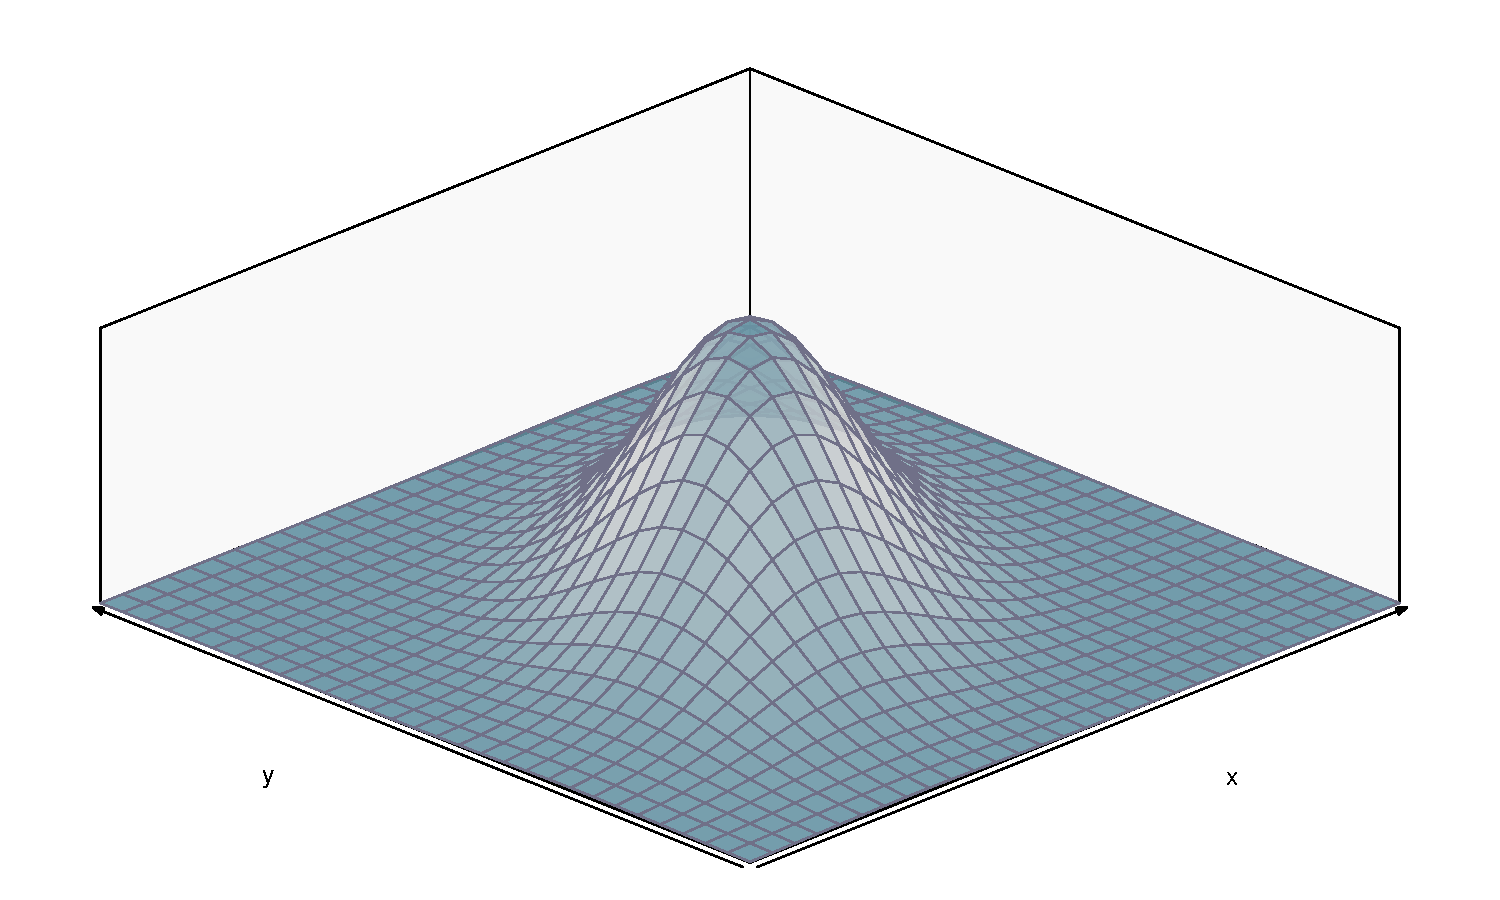
\includegraphics{Tema_4_VA_Continuas_multidimensionales_files/figure-beamer/unnamed-chunk-1-1} \end{center}
\end{frame}

\hypertarget{distribuciones-multidimensionales}{%
\section{Distribuciones
multidimensionales}\label{distribuciones-multidimensionales}}

\begin{frame}{Conceptos básicos. Función de probabilidad y de
distribución.}
\protect\hypertarget{conceptos-buxe1sicos.-funciuxf3n-de-probabilidad-y-de-distribuciuxf3n.}{}
Consideremos un vector compuesto de \(n\) variables aleatorias continuas
\((X_1,X_2,\ldots,X_n)\)

Su \textbf{función de densidad de probabilidad} es una función
\(f_{X_1,X_2,\ldots, X_n}:\mathbb{R}^n\mapsto [0,+\infty)\) tal que

\[F_{X_1,X_2,\ldots, X_n}(x_1,x_2,\ldots,x_n)=P(X_1\leq x1,X_2\leq x_2,\ldots, X_n\leq x_n)=\int_{-\infty}^{x1}\int_{-\infty}^{x2}\cdots \int_{-\infty}^{xn} f(t_1,t_3,\ldots,t_n)\quad dt_1 dt_2\cdots dt_n.\]
\end{frame}

\begin{frame}{Independencia}
\protect\hypertarget{independencia}{}
Definición independencia

Diremos que la variables continuas \(X_1,X_2,\ldots, X_n\) son
\textbf{INDEPENDIENTES} cuando
\[f_{X_1,X_2,\ldots, X_n}(x_1,x_2,\ldots,x_n) =f_{X_1}(x_1)\cdot f_{X_2}(x_2)\cdot  \ldots \cdot  f_{X_n}(x_n).\]

Propiedad

Las variables \(X_1,X_2,\ldots, X_n\) son \textbf{INDEPENDIENTES} si y
solo si
\[F_{X_1,X_2,\ldots, X_n}(x_1,x_2,\ldots,x_n)=F_{X_1}(x_1)\cdot F_{X_2}(x_2)\cdot  \ldots \cdot  F_{X_n}(x_n).\]
\end{frame}

\begin{frame}{Conceptos básicos}
\protect\hypertarget{conceptos-buxe1sicos}{}
Vector de medias

Si denotamos \(E(X_i)=\mu_i\) para \(i=1,2,\ldots,n\) el \textbf{vector
de medias} es
\[E(X_1,X_2,\ldots,X_n)=(E(X_1),E(X_2),\ldots,E(X_n))=(\mu_1,\mu_2,\ldots,\mu_n).\]

Covarianza y varianzas

Si denotamos \(\sigma_{ij}=Cov(X_i,X_j)\) para todo \(i,j\) en
\(1,2,\ldots n\) entonces tenemos que

\begin{itemize}
\tightlist
\item
  \(\sigma_{ii}=Cov(X_i,X_i)=\sigma_{ii}=\sigma_i^2.\)
\item
  \(\sigma_{ij}=Cov(X_i,X_j)=Cov(X_j,X_i)=\sigma_{ji}.\)
\end{itemize}
\end{frame}

\begin{frame}{Conceptos básicos}
\protect\hypertarget{conceptos-buxe1sicos-1}{}
Si denotamos \(\rho_{ij}=Cor(X_i,X_j)\) para todo \(i,j\) en
\(1,2,\ldots n\) entonces tenemos que

\begin{itemize}
\tightlist
\item
  \(\rho_{ii}=Cor(X_i,X_i)=1.\)
\item
  \(\rho_{ij}=Cor(X_i,X_j)=Cor(X_j,X_i)=\rho_{ji}.\)
\end{itemize}
\end{frame}

\begin{frame}{Matrices de varianzas-covarianzas y de correlaciones}
\protect\hypertarget{matrices-de-varianzas-covarianzas-y-de-correlaciones}{}
\[\Sigma=\pmatrix{ \sigma_{1}^2 & \sigma_{12} & \ldots & \sigma_{1n}\\
 \sigma_{21} & \sigma_{2}^2 & \ldots & \sigma_{2n}\\
 \vdots & \vdots & \ddots& \vdots\\
 \sigma_{n1} & \sigma_{n2} & \ldots & \sigma_{n}^2
 }, \qquad R=\pmatrix{ 1 & \rho_{12} & \ldots & \rho_{1n}\\
 \rho_{21} & 1 & \ldots & \rho_{2n}\\
 \vdots & \vdots & \ddots& \vdots\\
 \rho_{n1} & \rho_{n2} & \ldots & 1
 }.\]
\end{frame}

\end{document}
